\documentclass[../main.tex]{subfiles}

\begin{document}

\section{Component wiring schematics}

\subsection{Meeple}

It consists on 2 LEDs, a green one and a yellow one, a hall sensor, a microcontroller (ESP-01) and a battery, as in the \textbf{Figure \ref{fig:meeple}}. Each component has the following function:

\begin{enumerate}
    \item \textbf{ESP-01}: Microcontroller that controls the LEDs, reads the Hall Sensor and reads/writes feedback with MQTT.
    \item \textbf{Battery}: Power source for the ESP-01
    \item \textbf{Hall Sensor}: Detects when the meeple is being detected on board, detects meeple movement and death.
    \item \textbf{Green LED}: Has two modes, when blinking it indicates that it's the meeple turn for moving, when solid it indicates the hall sensor is detecting a magnetic field (the meeple is detecting the board).
    \item \textbf{Yellow LED}: Indicates if the player has the bullet on the shooting stage.
\end{enumerate}

\begin{figure}[!htb]
    \centering
    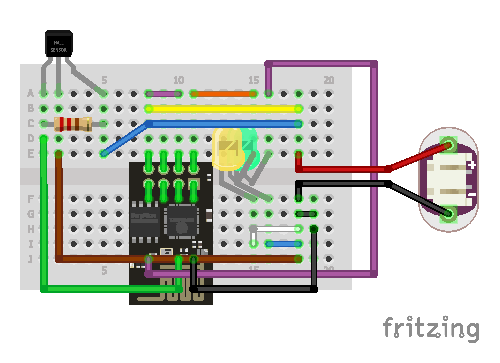
\includegraphics[width= 0.7\linewidth]{../media/figures/schematic_meeple.pdf}
    \caption{Meeple components schematic}
    \label{fig:meeple}
\end{figure}

\subsection{Operation base}

It consists on a red LED, a button, a buzzer, a microcontroller (ESP-32) and a LCD screen connected through a I2C module, as shown in the \textbf{Figure \ref{fig:base}}. Each component has the following function:

\begin{enumerate}
    \item \textbf{ESP-32}: Microcontroller that controls the LCD screen, reads the button, reads/writes feedback with MQTT (through WiFi) and controls the buzzer.
    \item \textbf{LCD screen}: Displays the current game stage and the player's turn.
    \item \textbf{Button}: Used to shoot the bullet.
    \item \textbf{Buzzer}: Indicates the end of the game.
    \item \textbf{Red LED}: Indicates whether the player has the bullet.
    \item \textbf{I2C module}: Module that connects the ESP-32 with the LCD screen through I2C protocol.
    \item \textbf{Resistors}: Both resistors are 220 Ohm and are used to limit the current.
\end{enumerate}

The board can be powered through a Micro-USB cable from a computer USB port.

\begin{figure}
    \centering
    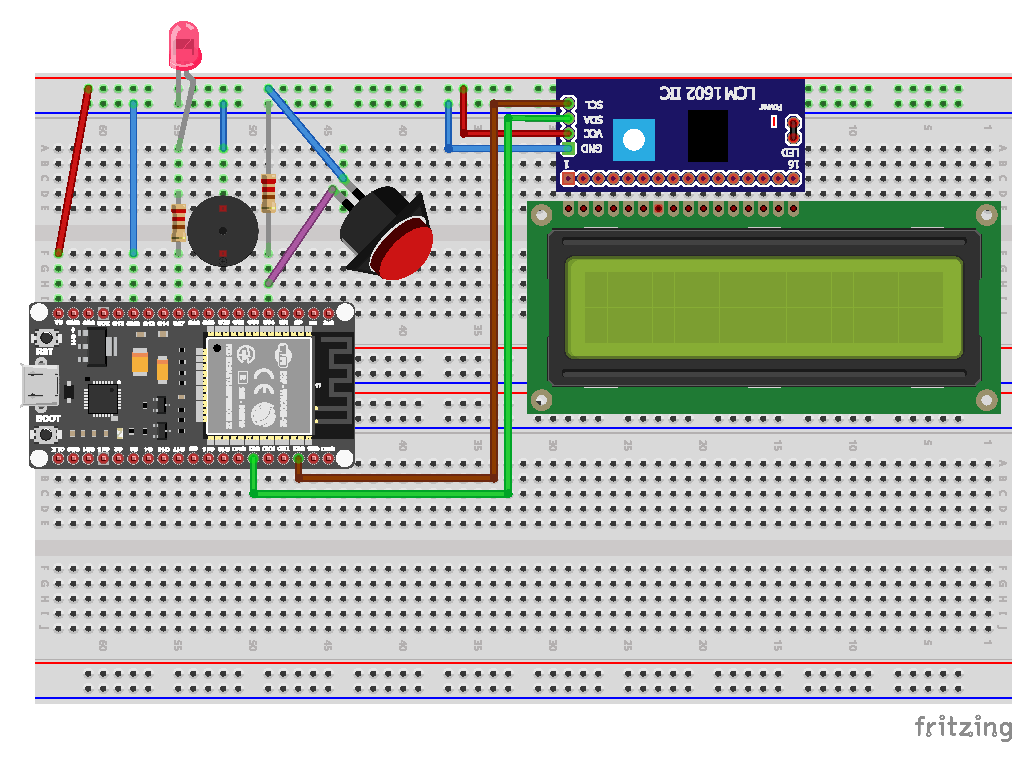
\includegraphics[width= 0.99\linewidth]{../media/figures/schematic_bb.pdf}
    \caption{Operation base components schematic}
    \label{fig:base}
\end{figure}

\end{document}